\documentclass{beamer}

\usefonttheme{professionalfonts} % using non standard fonts for beamer
\usefonttheme{serif} % default family is serif

\usepackage{hyperref}
%\usepackage{minted}
\usepackage{animate}
\usepackage{graphicx}
\def\Put(#1,#2)#3{\leavevmode\makebox(0,0){\put(#1,#2){#3}}}
\usepackage{colortbl}
\usepackage{tikz}
\usepackage{amssymb}
\usepackage{enumerate}
\usepackage{arydshln}
\usepackage{algorithm}
\usepackage{algpseudocode}

\colorlet{lightred}{red!25}
\colorlet{lightgreen}{green!25}
\beamertemplatenavigationsymbolsempty

\newcommand\blfootnote[1]{%
  \begingroup
  \renewcommand\thefootnote{}\footnote{#1}%
  \addtocounter{footnote}{-1}%
  \endgroup
}

\makeatletter

%% Textclass specific LaTeX commands.
\newcommand\makebeamertitle{\frame{\maketitle}}%
\AtBeginDocument{%
  \let\origtableofcontents=\tableofcontents
  \def\tableofcontents{\@ifnextchar[{\origtableofcontents}{\gobbletableofcontents}}
  \def\gobbletableofcontents#1{\origtableofcontents}
}
%% User specified LaTeX commands.
\usetheme{Malmoe}
\useoutertheme{infolines}
\addtobeamertemplate{headline}{}{\vskip2pt}
\setbeamercovered{transparent}

\makeatother

%%%%%%%%%%%%%%%%%%%%%%%%%%%%%%%%%%%%%%
%% Main document
%%%%%%%%%%%%%%%%%%%%%%%%%%%%%%%%%%%%%%
\begin{document}
\title[PFLOCK report]{PFLOCK Report}
\author[AC]{Andres Calderon}
\institute[Spring'20]{University of California, Riverside}
\makebeamertitle
\newif\iflattersubsect

\AtBeginSection[] {
    \begin{frame}<beamer>
    \frametitle{Outline} 
    \tableofcontents[currentsection]  
    \end{frame}
    \lattersubsectfalse
}

\AtBeginSubsection[] {
    \begin{frame}<beamer>
    \frametitle{Outline} 
    \tableofcontents[currentsubsection]  
    \end{frame}
}

\begin{frame}{Reducing number of candidate centers}{Overall approach}
    \begin{enumerate}
        \item Identify dense partitions:
        \begin{itemize}
            \item by number of connection at each point.
        \end{itemize}
        \item At each partition built local partitions:
        \begin{itemize}
            \item it can be done using DBScan or uniform grids.
        \end{itemize}
    \end{enumerate}

\end{frame}

\begin{frame}{Local - partitioning}{DBScan}
  \centering
  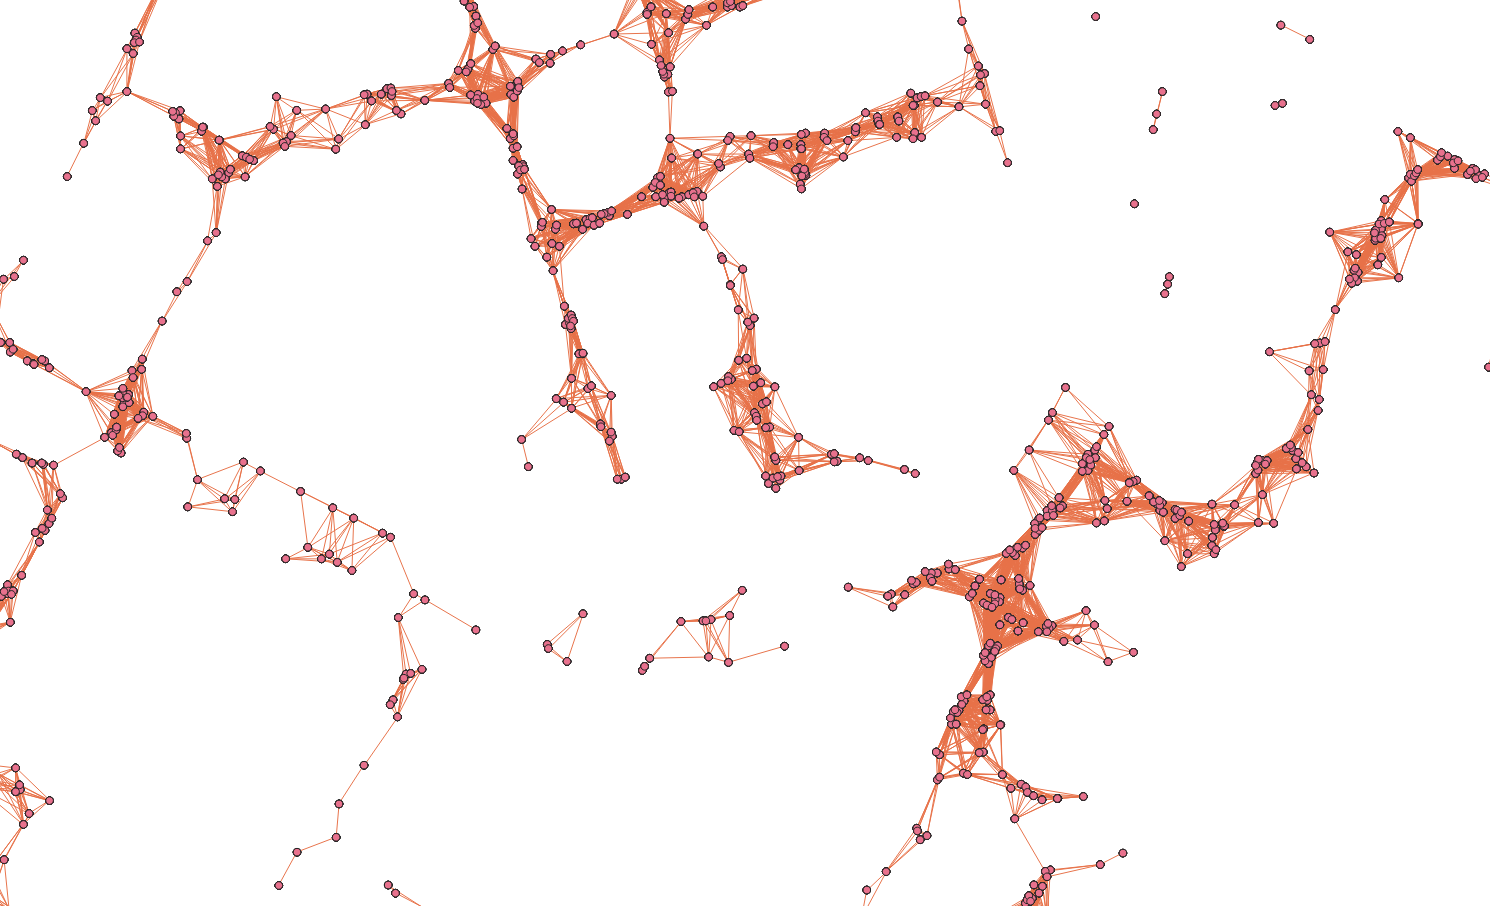
\includegraphics[width=0.9\textwidth]{figures/dbscan}
\end{frame}
\begin{frame}{Local - partitioning}{Uniform grids}
  \centering
  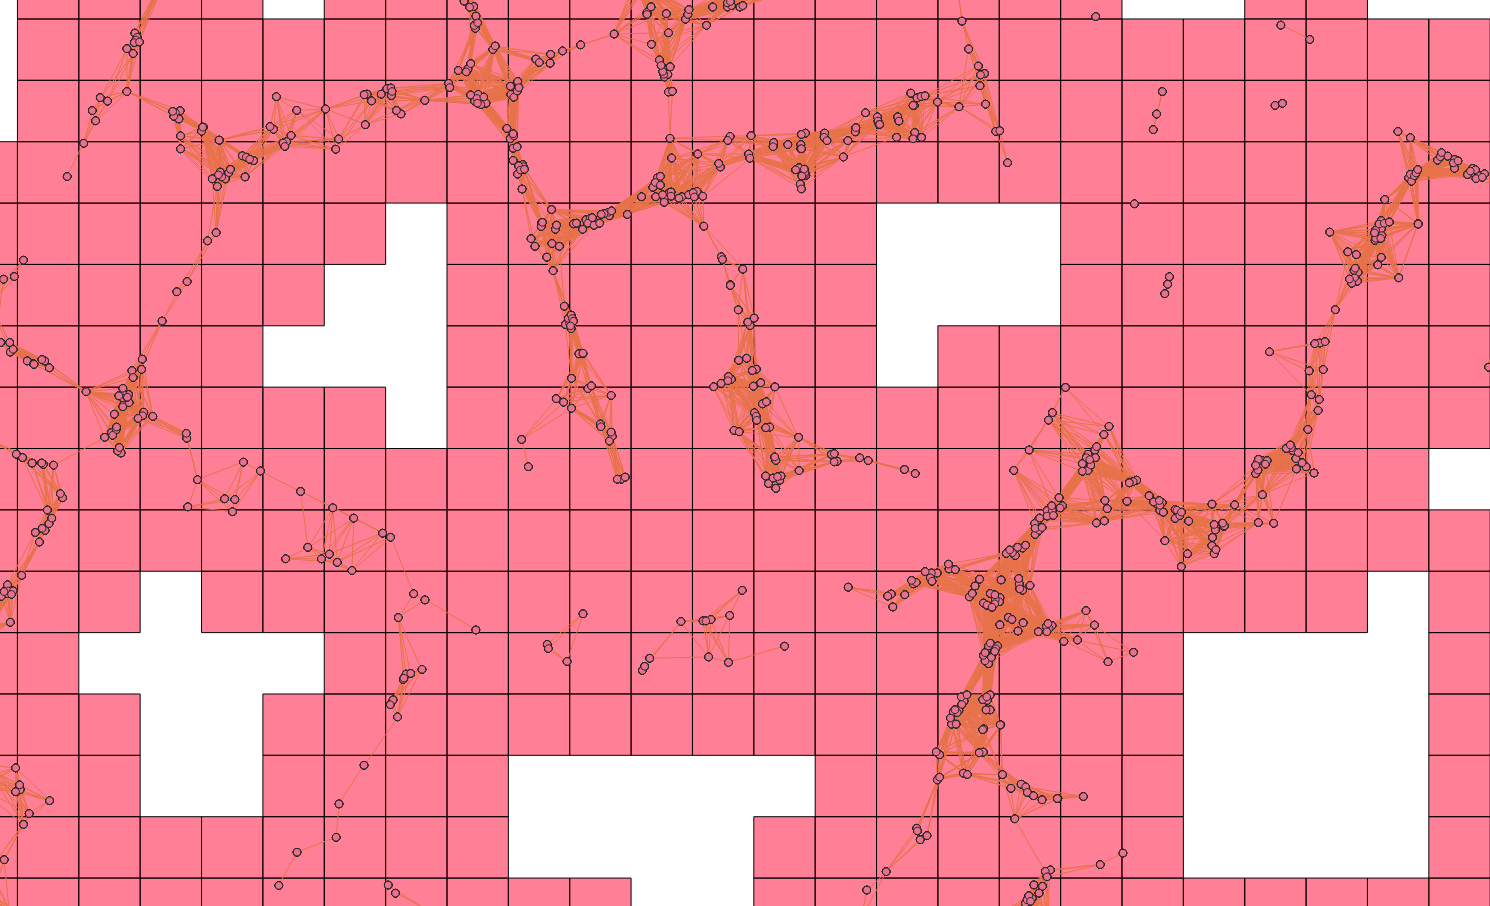
\includegraphics[width=0.9\textwidth]{figures/grids}
\end{frame}

\begin{frame}{Reducing number of candidate centers}{Overall approach}
    \begin{enumerate}
        \item Identify dense partitions:
        \begin{itemize}
            \item by number of connection at each point.
        \end{itemize}
        \item At each partition built local partitions:
        \begin{itemize}
            \item it can be done using DBScan or uniform grids.
        \end{itemize}
        \item For each local partition:
        \begin{enumerate}
            \item  If the farthest points distance $< epsilon$:
            \begin{itemize}
                \item retrieve centroid as unique center
            \end{itemize}
            \item  Find full set of triangles for the graph:
            \begin{itemize}
                \item retrieve the centroids of each triangle.
            \end{itemize}
        \end{enumerate}

    \end{enumerate}
\end{frame}

\begin{frame}{Centers by tringles}
  \centering
  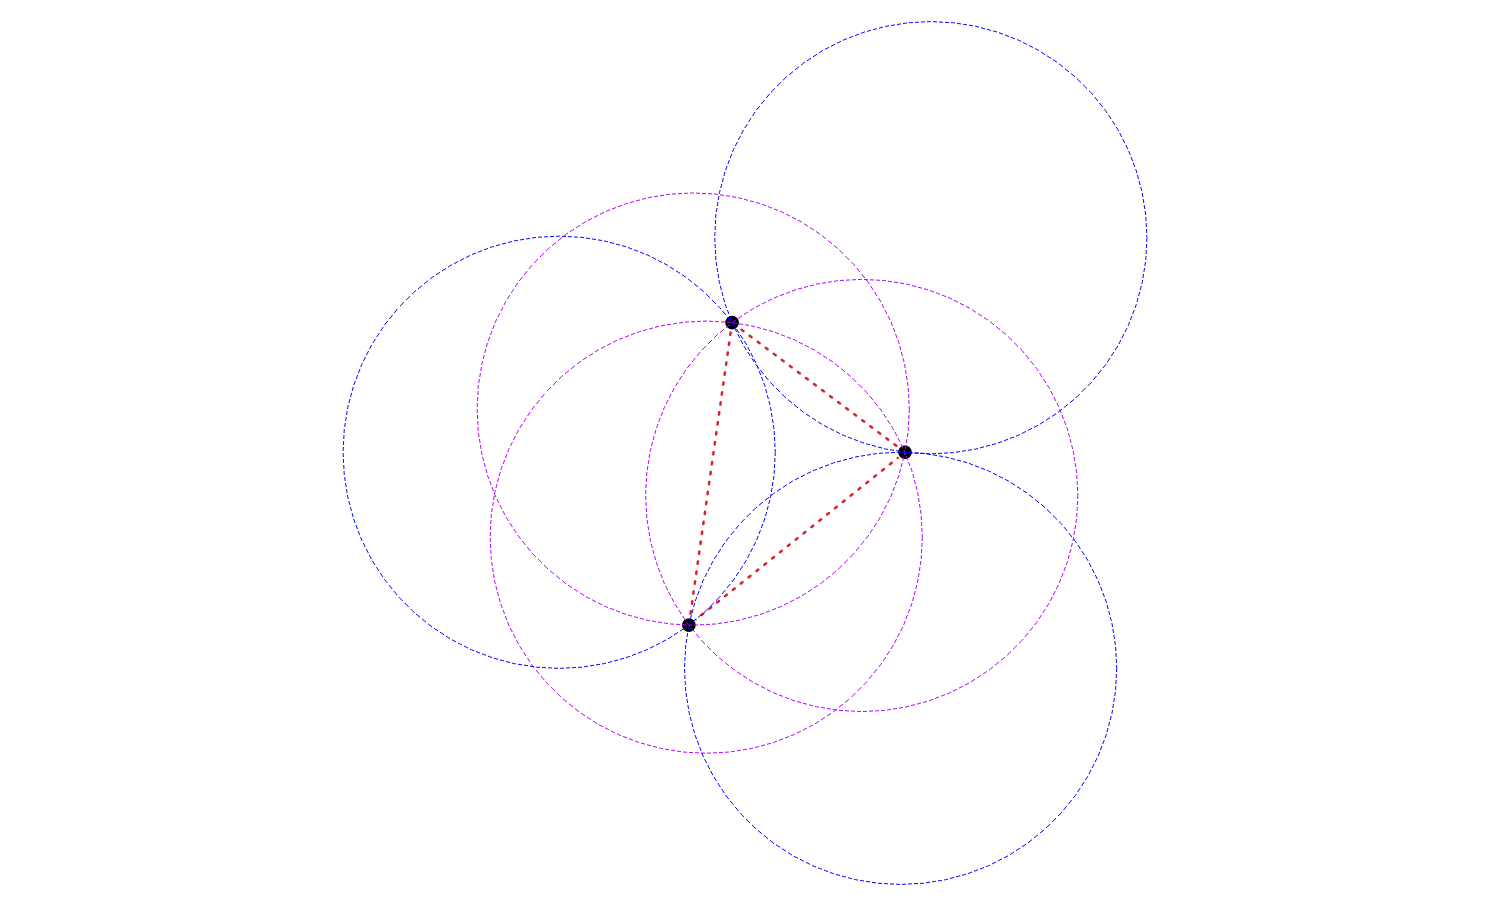
\includegraphics[width=0.9\textwidth]{figures/triangle1}
\end{frame}
\begin{frame}{Centers by tringles}
  \centering
  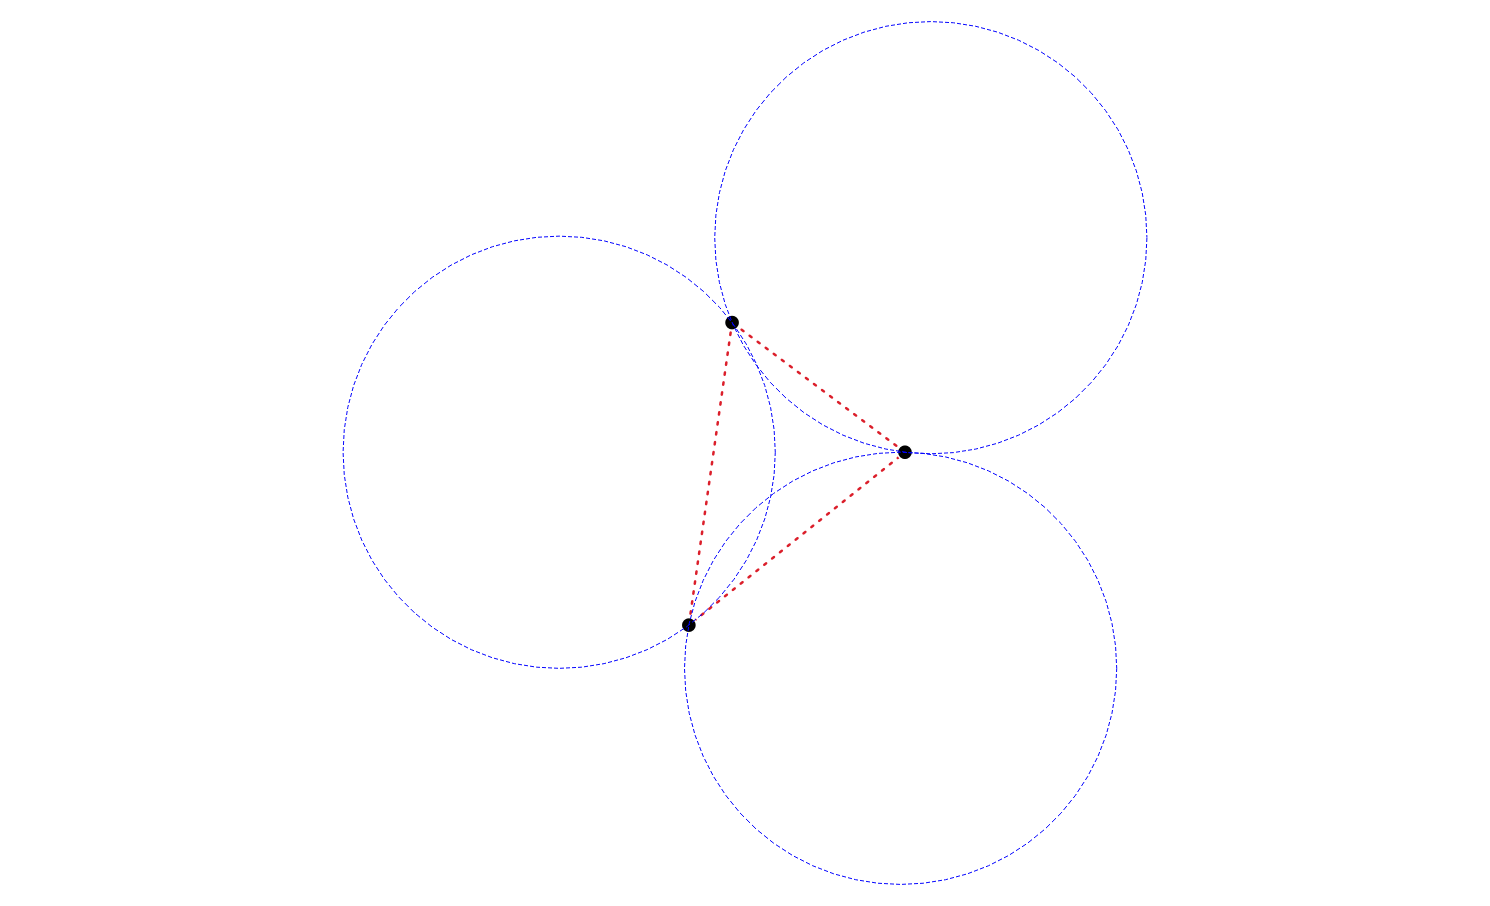
\includegraphics[width=0.9\textwidth]{figures/triangle2}
\end{frame}
\begin{frame}{Centers by tringles}
  \centering
  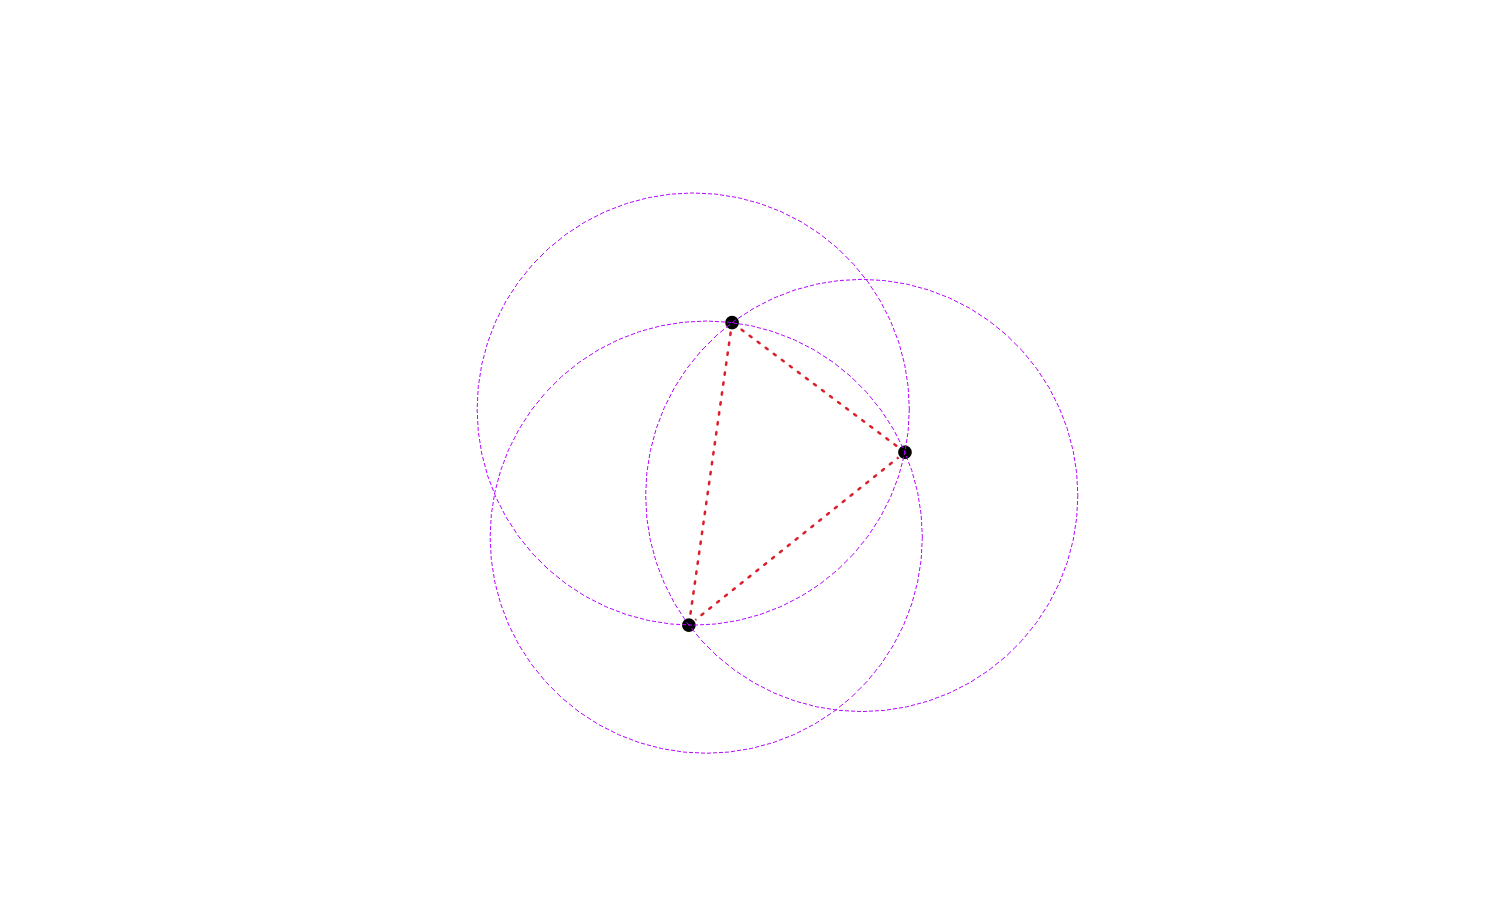
\includegraphics[width=0.9\textwidth]{figures/triangle3}
\end{frame}
\begin{frame}{Centers by tringles}
  \centering
  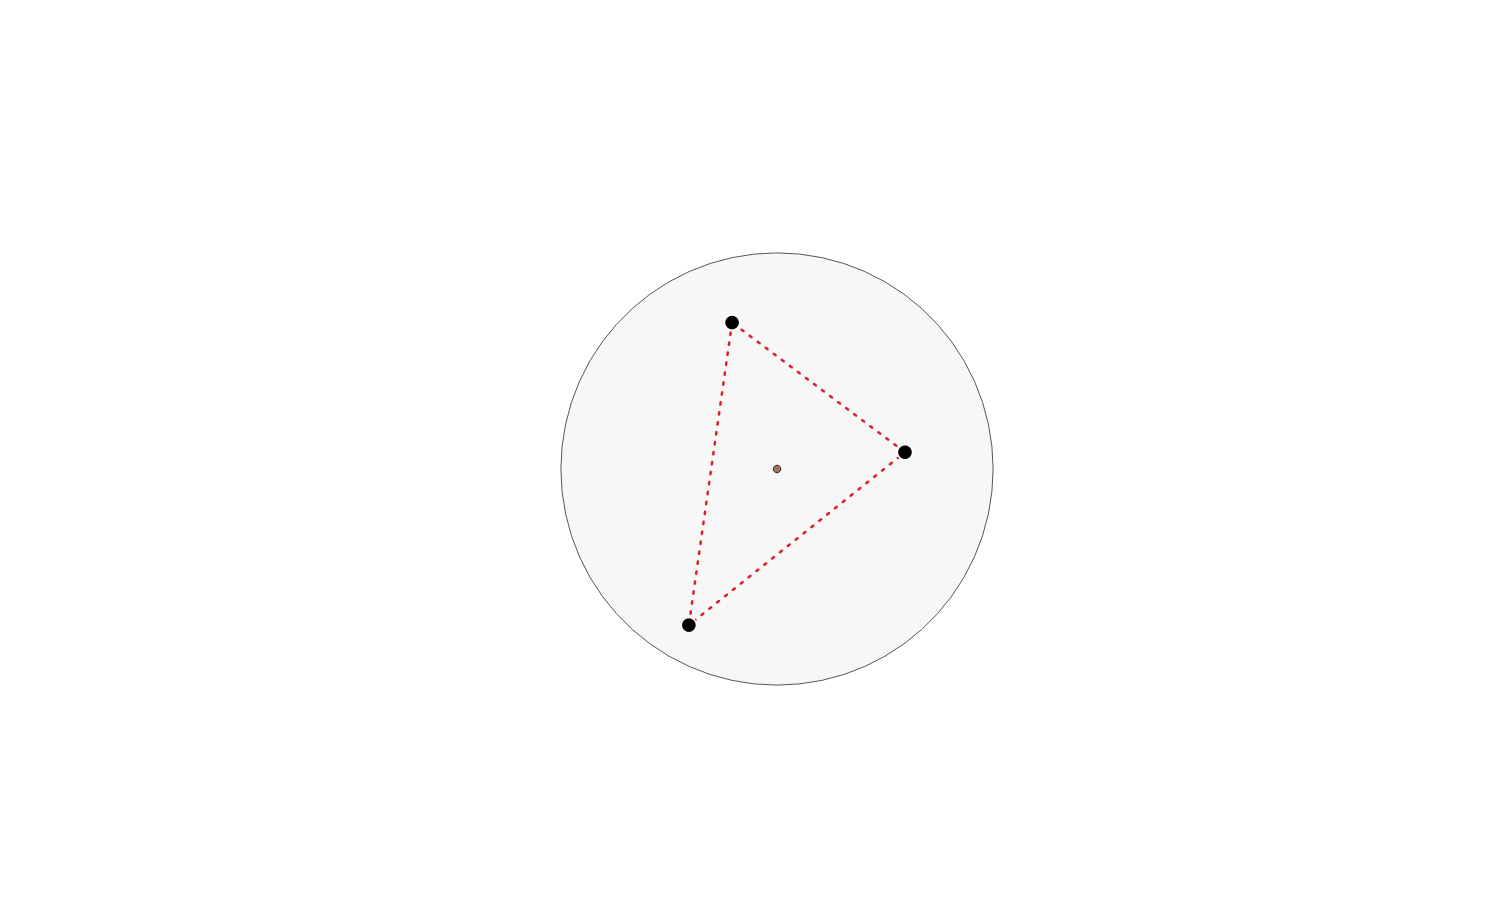
\includegraphics[width=0.9\textwidth]{figures/triangle4}
\end{frame}

\begin{frame}{Notes}
    \begin{itemize}
        \item We can use farthest point distance or smallest enclosing circle which can be done in linear-time.
        \item Find all the triangles on a graph is quite costly ($O(n^{1.5})$ in the number of edges), we will depends on a fine-grain partitions.
    \end{itemize}

\end{frame}


\end{document}

